
\fancyhead[R]{Leonie Boland}
\subsection{Deep Q-Learning Agent}

In this section we are giving an overview of the experiments we have done with our deep q-learning model that lead to our best performing agent. The basic framework is already described in the sections Methods and Training (give reference here). Hence at this point we trained the model, evaluated the performance and based upon that we changed hyperparameters or auxiliary rewards to improve the model.\\ \\
Initially, most experiments resulted in the fine tuning of the rewards and auxiliary reward functions. A good indication that the rewards are not helping the model to get trained in the most efficient way is a big deviation between the sum of the rewards in comparison to the score achieved by the agent. Ideally the score in the end of a round is constantly high if the sum of the rewards is high too, especially if the rewards' sum is in a high range for many rounds already, so if it has converged. The plots in Figure \ref{fig:rewardVSscore} show an contrary example of this phenomenon when the model was trained for 10000 rounds in the 7 $\times$ 7 coin heaven scenario. These plots do not show one straight line but a constantly changing reward sum respectively score on a high scale x-axis. This is why the plots come off rather chaotic than organized, but they still depict the training's progress. In this example there is a quite sudden improvement in the score between the 2000th and 3000th round of training and this jump can also be observed in the rewards plot on the left but is much less significant. Furthermore, the rewards still increase and seem to have converged after the 5000th round of training. Nonetheless the score is getting worse and keeps fluctuating between the highest possible score 21 and a score as low as 3. This means, that even though the model obviously has not found a good way for the agent to run in the coin heaven environment the rewards, that it is receiving, indicate exactly that the way the agent acts is good. When letting the agent play we noticed that this happened because the agent dropped many unnecessary bombs and thus killed itself occasionally, so the agent was not able to collect all the coins. However the total amount of rewards was still high because the agent was remunerated a lot for outrunning a bomb and was not punished for dropping a totally unnecessary bomb. We understood the background of this behavior by consulting the logged messages parallel to training the agent a few rounds with the GUI (Graphical User Interface) turned on. Therefore we fine tuned the rewards with a closer examination of matching the extent of rewards for different actions with each other. We also added a penalty for dropping bombs that will not destroy crates or are in reach of an opponent as described closely in section \ref{sec:deepqtraining}. 
\begin{figure}[H]
	\centering
	\begin{minipage}{0.49\textwidth}
		\centering
		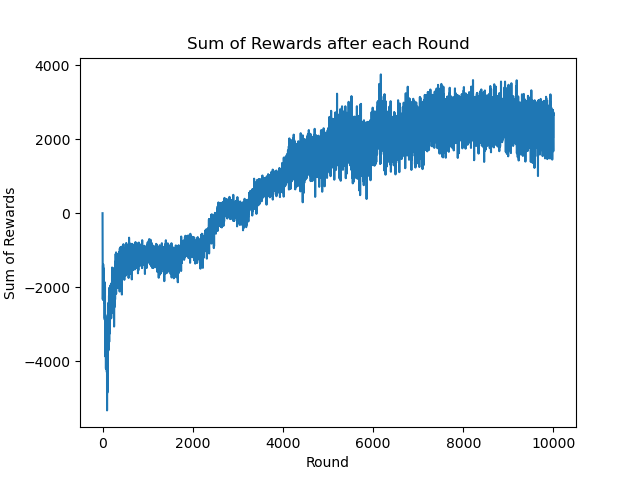
\includegraphics[scale=0.52]{images/rewards_converged.png}
	\end{minipage}
	\begin{minipage}{0.49\textwidth}
		\centering
		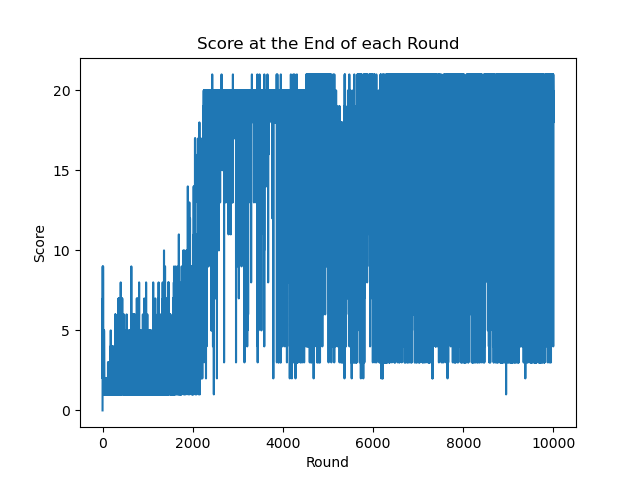
\includegraphics[scale=0.52]{images/scores_not_converged.png}
	\end{minipage}
	\caption{Both plots were generated during the training of the Deep Q-Model on a small coin-heaven scenario with coins on every free tile. The x-axis of both plots represents the rounds of the training. While the left plot depicts the sum of all rewards given to the agent in each round, the right plot shows the score after each round. These plots show discrepancy between rewards and scores.}
	\label{fig:rewardVSscore}
\end{figure}

After more test runs and improvements of the auxiliary rewards we were already able to produce a model that collected all coins efficiently. Figure \ref{fig:efficientCoinHeaven} shows the corresponding rewards and scores of 8000 rounds of training. This time score and reward coincide very well. Again, between the 2000th and 3000th round there is a steep increase of rewards and scores where the model apparently found a good way to handle this environment. Henceforward, both scores and rewards, are on a constantly high level. Of course, there is still a certain amount of fluctuation between each round as the agent is supposed to do some random moves during training to find a potentially better way of playing the game. Here the probability of doing a random move during training, not calculated by the network, was constantly 10\%.
\begin{figure}[H]
	\centering
	\begin{minipage}{0.49\textwidth}
		\centering
		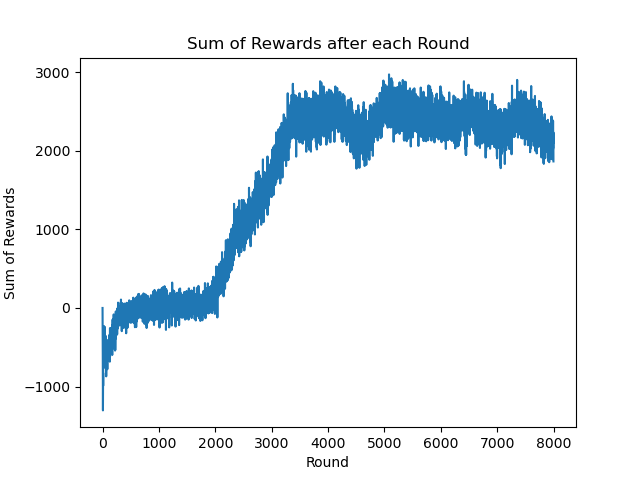
\includegraphics[scale=0.52]{images/rewards_perfect_coinheaven.png}
	\end{minipage}
	\begin{minipage}{0.49\textwidth}
		\centering
		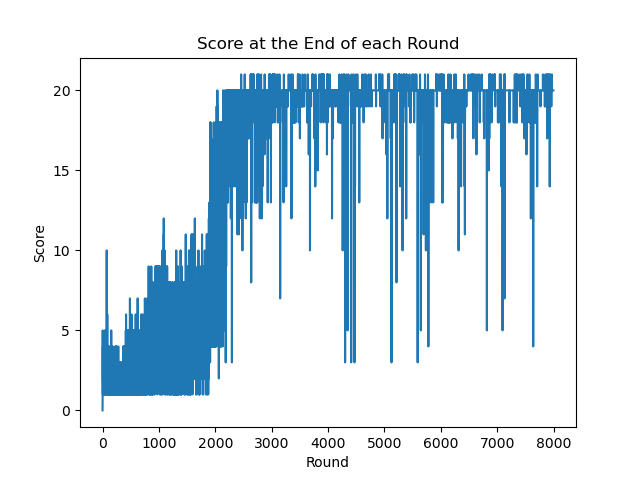
\includegraphics[scale=0.52]{images/scores_perfect_coinheaven.png}
	\end{minipage}
	\caption{The plots are constructed in the same way as described before, but after the reward fine-tuning. The scores shown here fit to the high reward sum.}
	\label{fig:efficientCoinHeaven}
\end{figure}

Although the auxiliary reward functions seemed to be elaborated very well at this point, the agent did not play smoothly on larger fields in the harder levels even after a lot of training rounds. The main concern was that the agent often kept killing itself in early steps of the game. With the assumption that the rewards are handed out reasonably we also had to evaluate other hyperparameters. Our neural network consisted of a very simple architecture so we thought about features to add to the network to enable better learning. Even though dropout is a very common property to have in neural networks, it did not make sense for our task as it is used to prevent overfitting, which cannot happen here. Instead we included batch normalization which should stabilize and accelerate the training \cite{batchnorm}. The batch normalization layers were placed before adding the four parallel models together as batch normalization after the concatenation normally leads to worse results \cite{batchnormpos}. Unfortunately when doing the training from scratch the batch normalization did not result in a better running agent or a faster training, probably because the batch size was too small. Not only was the batch size small in general with 256, but we could not collect enough training samples if the agent killed itself early in the game. This did not allow the positive effects of batch normalization to unfold in our network. Furthermore batch normalization is more efficient in deeper networks \cite{batchnorm}, but with one hidden layer our neural network is rather shallow.

Next we gave different loss functions a try. We initially used the smooth L1 loss but also thought of trying the cross-entropy loss because it is the standard loss for classification models, where the output usually is a list of probabilities. In our case the output gives the probability of an action to be the best action to take in the current state of the game for every possible action. Applying the cross-entropy loss showed that our model is not suited for this kind of loss. A reason for this could be that we want to find a good metric to calculate the loss between the predicted and the target q value, calculated following the Bellman equation. The literature hints that we should minimize the quadratic error between those values. In the formula for the cross-entropy loss presented in section \ref{sec:crossentropy} the quadratic error is not calculated. Instead, loss functions that can be considered next to the Smooth L1 loss is the closely related Huber loss and of course the MSE loss. In the end the MSE loss proofed to be most efficient, so our final agent was also trained with this loss. When discussing the loss we also inevitably gave thought to the optimizer. The AdamW optimizer worked well but RMSprop was more effective. Especially the faster convergences shown in Figure \ref{fig:adamvsrmsprop} was a decisive point in favor for the RMSprop optimizer. Thus we proceeded with RMSprop, but as AdamW achieved good results too, we believe that an agent trained with this optimizer would haven been able to run similarly when giving more consideration to the learning rate.
\begin{figure}[H]
	\centering
	\begin{minipage}{0.49\textwidth}
		\centering
		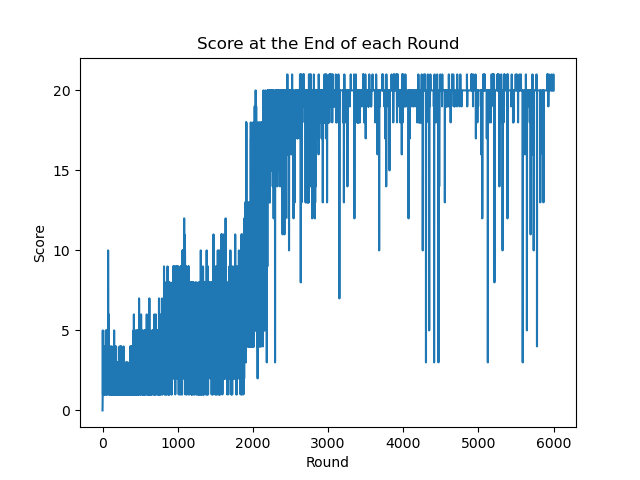
\includegraphics[scale=0.52]{images/scores_adamw.png}
	\end{minipage}
	\begin{minipage}{0.49\textwidth}
		\centering
		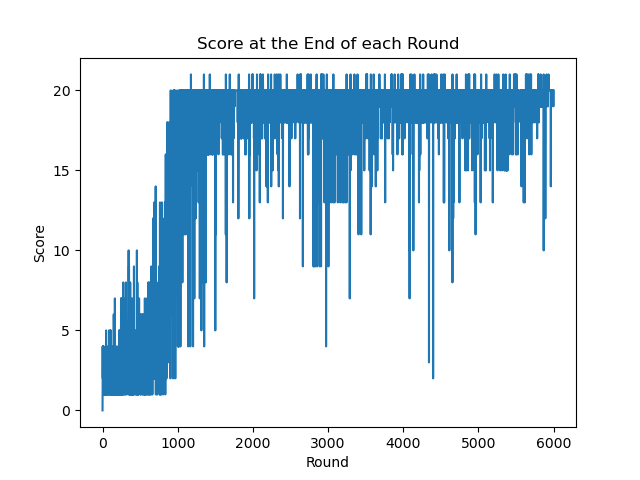
\includegraphics[scale=0.52]{images/scores_rmsprop.png}
	\end{minipage}
	\caption{The plots are constructed in the same way as before, but both plots depict the scores of to different trainings. The left one was trained with the optimizer AdamW and the right one was trained with RMSprop. The model using RMSprop improves and converges faster.}
	\label{fig:adamvsrmsprop}
\end{figure}

With the configurations chosen as explained above we reached a fairly good playing agent after 6000 rounds of training in coin heaven (7 $\times$ 7 field, coins on every free tile and 60 steps per round), 60000 rounds of training in loot crate (11 $\times$ 11 field, 20 coins, 0.4 crate density, 120 steps per round), 15000 rounds of training in classic (17 $\times$ 17 field, 9 coins, 0.75 crate density, 200 steps per round) and 40000 rounds of training in the classic scenario as described before but with two rule based agents and one coin collector agent as opponent. Strangely, except of being able to play the game well the agent did not learn to not do invalid actions. We observed that the majority of self killing happened because the agent still did invalid action, like trying to move in a direction, where a wall is located, to escape a bomb. Thus, to get a better playing agent we force the agent to not do invalid actions in the not-training mode. After each neural network output we check if the chosen action, so the action with the highest probability, can be executed and if not we take the action with the second highest probability and check this one. This is done until a valid action is found. 

Finally, we created an agent that can compete with a rule based and coin collector agent but is mostly not able to beat them. Still, we can conclude that our model did learn how to play the game as it clearly outperforms a random agent, which nearly always makes 0 points. Figure \ref{fig:game1} shows the scores of four agents, namely our reinforcement learning agent, a rule based agent, a coin collector agent and a random agent, when they play against each other in the classic scenario for 10 rounds. We also found that our agent performs better against stronger agents, maybe because it was trained against strong agents. When we choose the same opponents as during training, so 2 rule based agents and 1 coin collector, our agent often outperforms at least one of them.
\begin{figure}[H]
	\centering
	\begin{minipage}{0.49\textwidth}
		\centering
		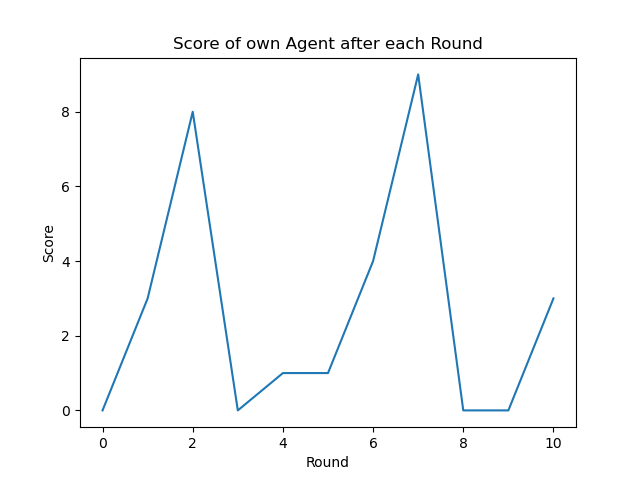
\includegraphics[scale=0.52]{images/my_scores11_1.png}
	\end{minipage}
	\begin{minipage}{0.49\textwidth}
		\centering
		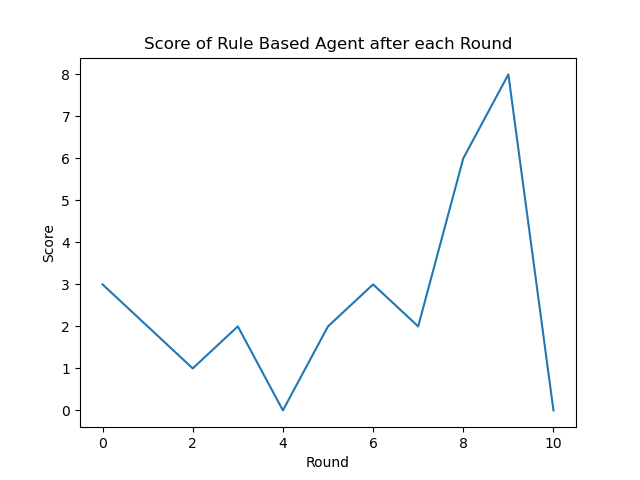
\includegraphics[scale=0.52]{images/rule_scores11_1.png}
	\end{minipage}
	\begin{minipage}{0.49\textwidth}
		\centering
		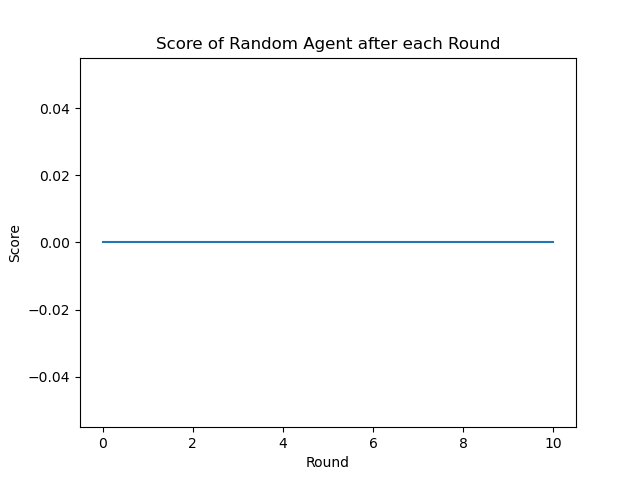
\includegraphics[scale=0.52]{images/random_scores11_1.png}
	\end{minipage}
	\begin{minipage}{0.49\textwidth}
		\centering
		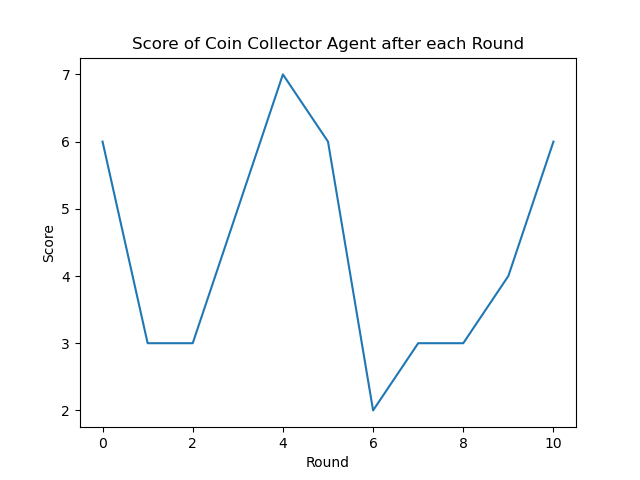
\includegraphics[scale=0.52]{images/coin_scores11_1.png}
	\end{minipage}
	\caption{These plots result from one game of bomberman with 10 rounds. Our reinforcement learning agent represented in the top left, played against a rule based agent represented in the top right, a coin collector agent represented in the bottom right and a random agent represented in the bottom left. While the random agent did not score any points, our agent and the rule based agent both scored 29 points in total and the coin collector won with 46 points.}
	\label{fig:game1}
\end{figure}

Currently our agent still has a few problems when playing the game. It kills itself sometimes by not escaping or escaping in a direction where the agent cannot get to safety. In consideration of our auxiliary rewards explained in section \ref{sec:rewards} this is a phenomenon that we did not expect as the auxiliary rewards are designed exactly to avoid this. Thus we hoped that the agent would learn quite early how to escape its own bombs. So unfortunately, due to time restrictions, we could not test whether more training solves the problem but we assume that it would not. This leaves us with the believe that there are still flaws in our model, the state to feature function or the auxiliary rewards. (VIELLEICHT EHER IN CONCLUSION?). Another undesired behavior is that the agent sometimes just stops moving even though there are still crates to destroy and coins to collect. Instead of stop moving it also sometimes gets caught in a loop, like just moving up and down all the time. All the same, the agent still escapes a bomb that is dropped by an opponent when it is too close. Sometimes we also observe that this can trigger the agent to move efficiently again. One reason for that could be that in our state to feature function we gave the agent only a 7 $\times$ 7 vision field with all the details it needs about crates, coins, opponents and bombs. We expected this to be a problem from the beginning so we included our so called outside map collecting information happening outside of this vision field, so that the agent still knows what is going on farther away. Probably this still is not enough to keep the agent moving especially as it is only directly rewarded for any movement if it is getting closer to a coin. Nonetheless it should be worthwhile for the agent to move towards crates and destroy them in the long run. Maybe this is a behavior that could be improved by more training even though the reward plots seem to show some convergence we never know if there could happen another positive adjustment to the agent after more training rounds.
